%\documentclass[ journal ]{new-aiaa}
\documentclass[conf]{new-aiaa}
\usepackage[utf8]{inputenc}
\usepackage{textcomp}
\usepackage{subfigure}
\usepackage{graphicx}
\usepackage{amsmath}
\usepackage[version=4]{mhchem}
\usepackage{siunitx}
\usepackage{longtable,tabularx}
\usepackage{cancel}

\setlength\LTleft{0pt} 

\begin{document}


\begin{figure}[hbt!]
    \centering
    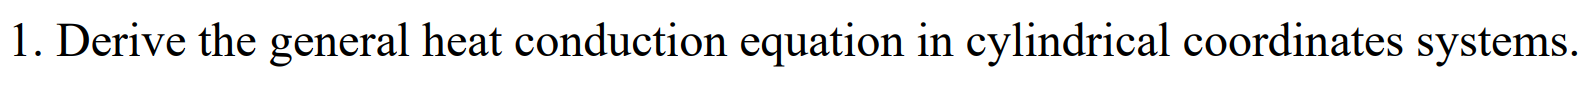
\includegraphics[width=1\textwidth]{problems/p1.png}
    \label{fig:p1}
\end{figure}
\begin{figure}[hbt!]
    \centering
    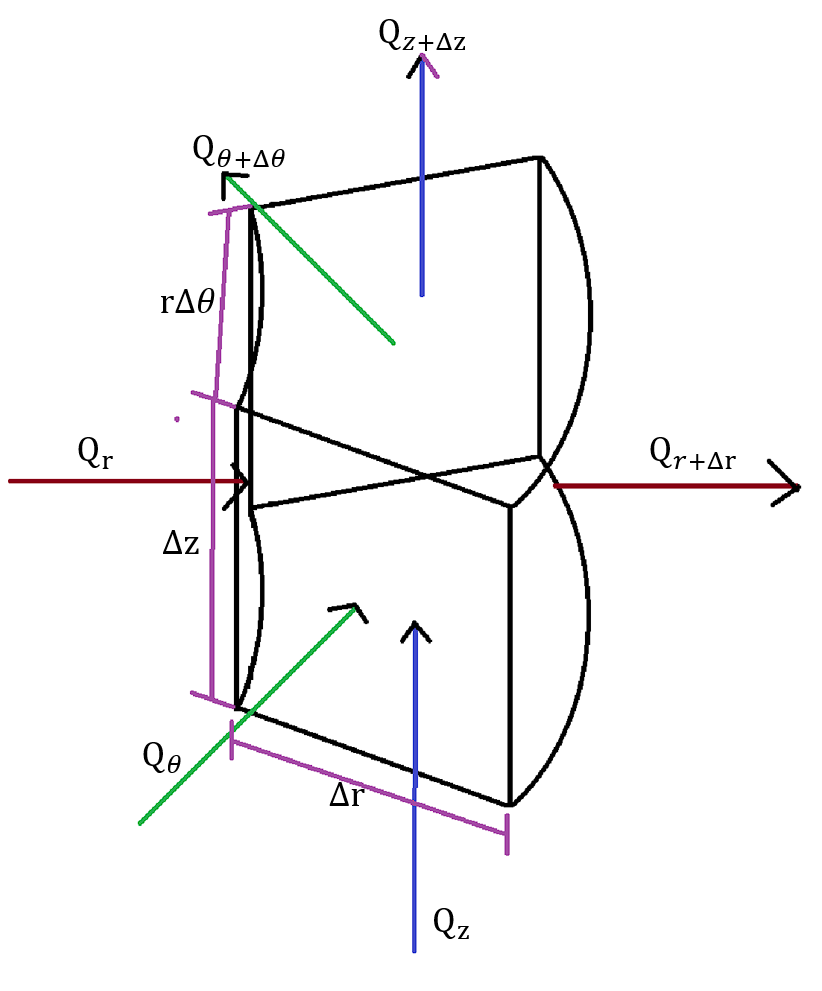
\includegraphics[width=0.5\textwidth]{problems/cyl_vol.png}
    \label{fig:p1}
\end{figure}

Start with a first law analysis of a single cylindrical element. This includes the energy entering the element, the energy leaving the element, and the energy generated within the element. 
Putting these together can give us the change in internal energy with respect to time:

\begin{equation*}
    \left(\dot{Q}_{r}-\dot{Q}_{r+\Delta r}\right)+\left(\dot{Q}_{\theta}-\dot{Q}_{\theta+\Delta \theta}\right)+\left(\dot{Q}_{z}-\dot{Q}_{z+\Delta z}\right) + \dot{E}_{gen,element} = \frac{\Delta E_{element}}{\Delta t}
\end{equation*}

\noindent Where:
\begin{equation*}
    \Delta E_{element} = E_{t+\Delta T} - E_t = m c \left(T_{t+\Delta t}+T_{t}\right) = \rho \Delta V c \left(T_{t+\Delta t}+T_{t}\right) = \rho \left[r\Delta r \Delta \theta \Delta z\right] c \left(T_{t+\Delta t}+T_{t}\right) 
\end{equation*}

\begin{equation*}
    \lim_{\Delta T \rightarrow 0} \frac{\Delta E_{element}}{\Delta T}
    = \rho \left[r\Delta r \Delta \theta \Delta z\right] c \frac{\partial T}{\partial t}
\end{equation*}

\begin{equation*}
    \dot{E}_{gen,element} = \frac{\dot{e}_{gen}}{\Delta V} = \frac{\dot{e}_{gen}}{r\Delta r \Delta \theta \Delta z}
\end{equation*}

\noindent Substituting gives:

\begin{equation*}
    \left(\dot{Q}_{r}-\dot{Q}_{r+\Delta r}\right)+\left(\dot{Q}_{\theta}-\dot{Q}_{\theta+\Delta \theta}\right)+\left(\dot{Q}_{z}-\dot{Q}_{z+\Delta z}\right) + 
    \frac{\dot{e}_{gen}}{r\Delta r \Delta \theta \Delta z} 
    = \rho \left[r\Delta r \Delta \theta \Delta z\right] c \frac{\partial T}{\partial t}
\end{equation*}

\noindent Now divide both sides by volume:

\begin{equation*}
    \frac{1}{r \Delta \theta \Delta z}  \frac{\dot{Q}_{r}-\dot{Q}_{r+\Delta r}}{\Delta r}
    +\frac{1}{r \Delta r \Delta z} \frac{\dot{Q}_{\theta}-\dot{Q}_{\theta+\Delta \theta}}{\Delta \theta}
    +\frac{1}{r \Delta r \Delta \theta} \frac{\dot{Q}_{z}-\dot{Q}_{z+\Delta z}}{\Delta z} 
    + \dot{e}_{gen} 
    = \rho c \frac{\partial T}{\partial t}
\end{equation*}

\noindent Now by taking the limit in each direction and applying Fourier's law of conduction:
\begin{equation*}
    \lim_{\Delta r \rightarrow 0}
    \frac{1}{r \Delta \theta \Delta z}  \frac{\dot{Q}_{r}-\dot{Q}_{r+\Delta r}}{\Delta r}
    = \frac{1}{r \Delta \theta \Delta z} \frac{\partial \dot{Q}_r}{\partial r}
    = \frac{1}{r \Delta \theta \Delta z} \frac{\partial}{\partial r} \left[-k r \Delta \theta \Delta z \frac{\partial T}{\partial r}\right]
    = \frac{1}{r} \frac{\partial}{\partial r} \left[-k r \frac{\partial T}{\partial r}\right]
\end{equation*}


\begin{equation*}
    \lim_{\Delta \theta \rightarrow 0}
    \frac{1}{r \Delta r \Delta \theta} \frac{\dot{Q}_{\theta}-\dot{Q}_{\theta+\Delta \theta}}{\Delta \theta}
    = \frac{1}{\Delta r \Delta z} \frac{\partial \dot{Q}_{\theta}}{r \partial \theta}
    = \frac{1}{\Delta r \Delta z} \frac{\partial}{r \partial \theta}\left[-k\Delta r \Delta z \frac{\partial T}{ r \partial \theta}\right]
    = \frac{1}{r^2} \frac{\partial}{\partial \theta}\left[-k \frac{\partial T}{ \partial \theta}\right]
\end{equation*}

\begin{equation*}
    \lim_{\Delta z \rightarrow 0}
    \frac{1}{ r \Delta r \Delta \theta} \frac{\dot{Q}_{z}-\dot{Q}_{z+\Delta z}}{r \Delta z}
    = \frac{1}{ r \Delta r \Delta \theta} \frac{\partial \dot{Q}_{z}}{\partial z}
    = \frac{1}{ r \Delta r \Delta \theta} \frac{\partial}{\partial z}\left[-k r \Delta r \Delta \theta \frac{\partial T}{\partial z}\right]
    = \frac{\partial }{\partial z} \left[ -k \frac{\partial T}{\partial z}\right]
\end{equation*}

\noindent Substituting back into the main equation gives:

\begin{equation*}
    \frac{1}{r} \frac{\partial}{\partial r} \left[-k r \frac{\partial T}{\partial r}\right]
    + \frac{1}{r^2} \frac{\partial}{\partial \theta}\left[-k \frac{\partial T}{ \partial \theta}\right]
    + \frac{\partial }{\partial z} \left[ -k \frac{\partial T}{\partial z}\right]
    + \dot{e}_{gen} 
    = \rho c \frac{\partial T}{\partial t}
\end{equation*}

\noindent Now dividing by the thermal conductivity and simplifying gives:

\begin{equation*}
    \boxed{\frac{1}{r} \frac{\partial}{\partial r} \left(r \frac{\partial T}{\partial r}\right) + \frac{1}{r^{2}} \frac{\partial^2 T}{\partial \theta^2}+\frac{\partial^2 T}{\partial Z^2}+ \frac{\dot{e_{gen}}}{k} = \frac{1}{\alpha} \frac{\partial T}{\partial t}}
\end{equation*}

%
%
%  Problem 2
%
%
\pagebreak 
\begin{figure}[hbt!]
    \centering
    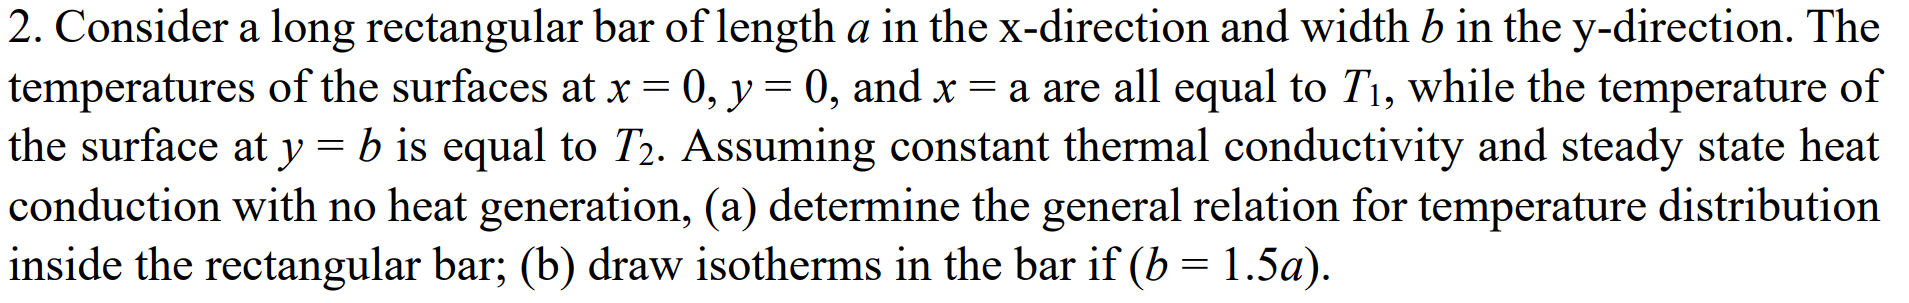
\includegraphics[width=1\textwidth]{problems/p2.png}
    \label{fig:p2}
\end{figure}





\begin{figure}[hbt!]
    \centering
    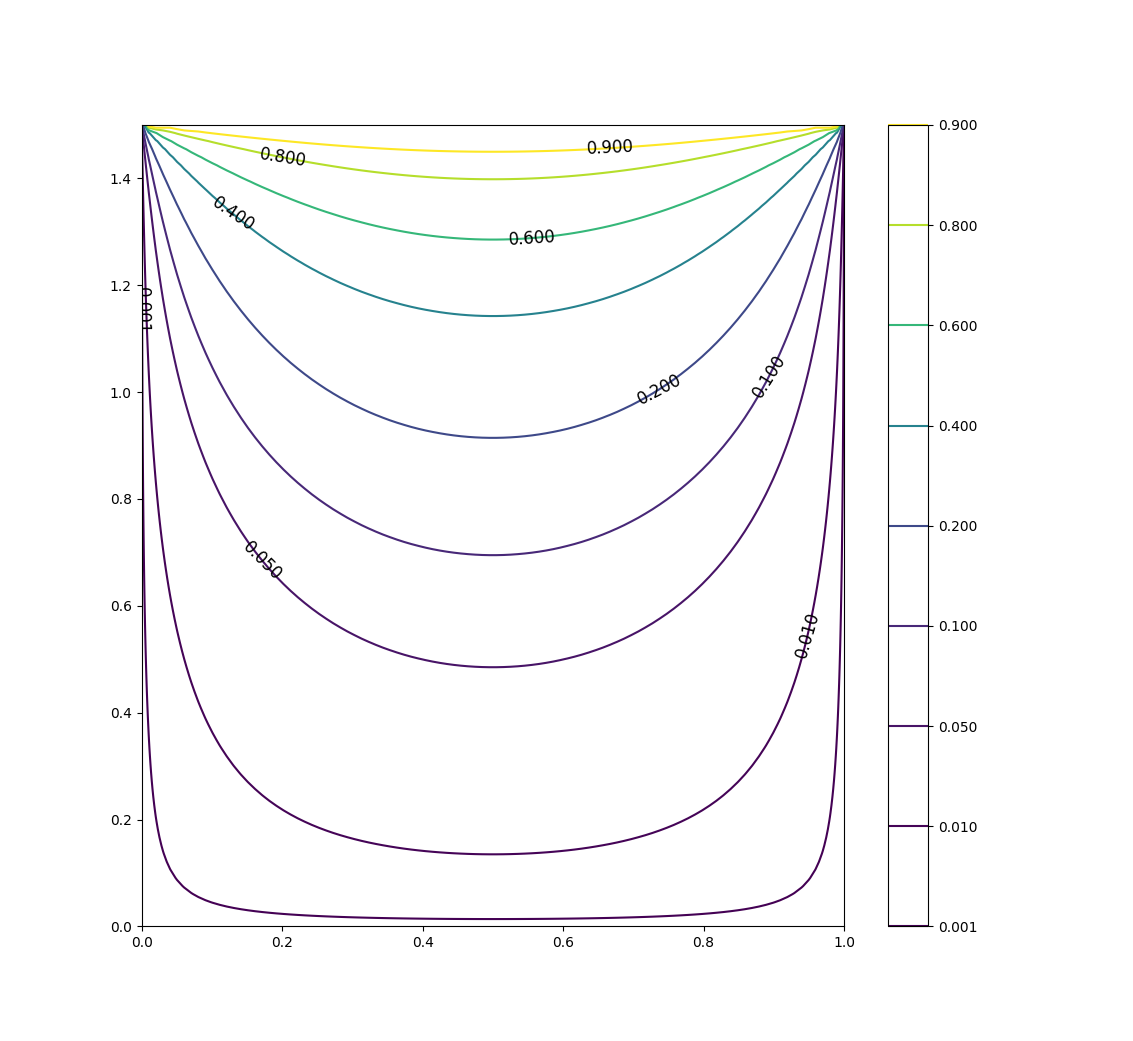
\includegraphics[width=1\textwidth]{plot/2D_conductionpng.png}
    \label{fig:2D_cond}
\end{figure}




%
%
%  Problem 3
%
%
\pagebreak 
\begin{figure}[hbt!]
    \centering
    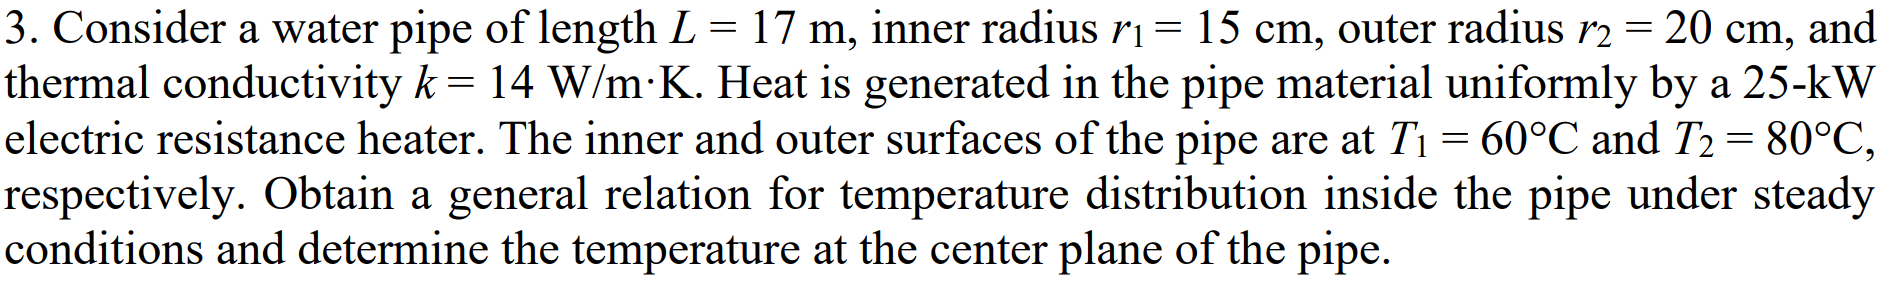
\includegraphics[width=1\textwidth]{problems/p3.png}
    \label{fig:p3}
\end{figure}

\noindent Energy generation rate per unit volume is:
\begin{equation*}
    \dot{e}_{gen} = \frac{\dot{E}_{gen}}{V} = \frac{\dot{E}_{gen}}{\pi \left(r_2^2 - r_1^2\right) L}
    = \frac{25000}{\pi \left({0.20}^2 - {0.15}^2\right) 17}
    = 26748.730  \frac{W}{m^3}
\end{equation*}

\noindent 1D heat transfer equation for a long tube at steady state:
\begin{equation*}
    \frac{1}{r} \frac{\partial}{\partial r}\left(r \frac{\partial T}{\partial r}\right) + \frac{\dot{e_{gen}}}{k}= 0
\end{equation*}

\begin{equation*}
    \Rightarrow \frac{\partial}{\partial r}\left(r \frac{\partial T}{\partial r}\right) = - r \frac{\dot{e_{gen}}}{k}
\end{equation*}


\noindent Integrating with respect to radius gives:
\begin{equation*}
    r \frac{\partial T}{\partial r} = - r^2 \frac{\dot{e_{gen}}}{2k} + c_1
\end{equation*}

\begin{equation*}
    \Rightarrow \frac{\partial T}{\partial r} = - r \frac{\dot{e_{gen}}}{2k} + \frac{c_1}{r}
\end{equation*}

\noindent Integrating again with respect to the radius gives:
\begin{equation*}
    T(r) = - r^2 \frac{\dot{e_{gen}}}{4k} + c_1 \ln r + c_2
\end{equation*}

\noindent Apply the boundary conditions:
\begin{equation*}
    T(r_1) = T_1 = - {r_1}^2 \frac{\dot{e_{gen}}}{4k} + c_1 \ln {r_1} + c_2
\end{equation*}
\begin{equation*}
    \Rightarrow c_2 = T_1 + {r_1}^2 \frac{\dot{e_{gen}}}{4k} - c_1 \ln {r_1} 
\end{equation*}
    
\begin{equation*}
    T(r_2) = T_2 = - {r_2}^2 \frac{\dot{e_{gen}}}{4k} + c_1 \ln {r_2} + c_2
\end{equation*}
\begin{equation*}
\Rightarrow c_2 = T_2 + {r_2}^2 \frac{\dot{e_{gen}}}{4k} - c_1 \ln {r_2} 
\end{equation*}


\begin{equation*}
    \Rightarrow T_1 + {r_1}^2 \frac{\dot{e_{gen}}}{4k} - c_1 \ln {r_1}
    = T_2 + {r_2}^2 \frac{\dot{e_{gen}}}{4k} - c_1 \ln {r_2} 
\end{equation*}

\begin{equation*}
    \Rightarrow  c_1 = \frac{T_2 - T_1 + \frac{\dot{e}_{gen}}{4k}\left(r_2^2 - r_1^2\right)} {\ln\frac{r_2}{r_1}} 
    = \frac{80 - 60 + \frac{26748.730}{4\times14}\left(0.20^2 - 0.15^2\right)} {\ln\frac{0.20}{0.15}}
    = 98.577
\end{equation*}

\begin{equation*}
    \Rightarrow c_2 = \left(80+273\right) + {0.2}^2 \frac{26748.730}{4\times14} - 98.577 \ln {0.2} = 530.911
    \end{equation*}

\noindent Now solving for the temperature at the midplane:
\begin{equation*}
    T(0.175) = - 0.175^2 \frac{26748.730}}{4\times14} + 98.577 \ln 0.175 + 530.911 = \boxed{344.46 K = 71.46 ^{\circ}C}
\end{equation*}
%
%
%  Problem 4
%
%
\pagebreak 
\begin{figure}[hbt!]
    \centering
    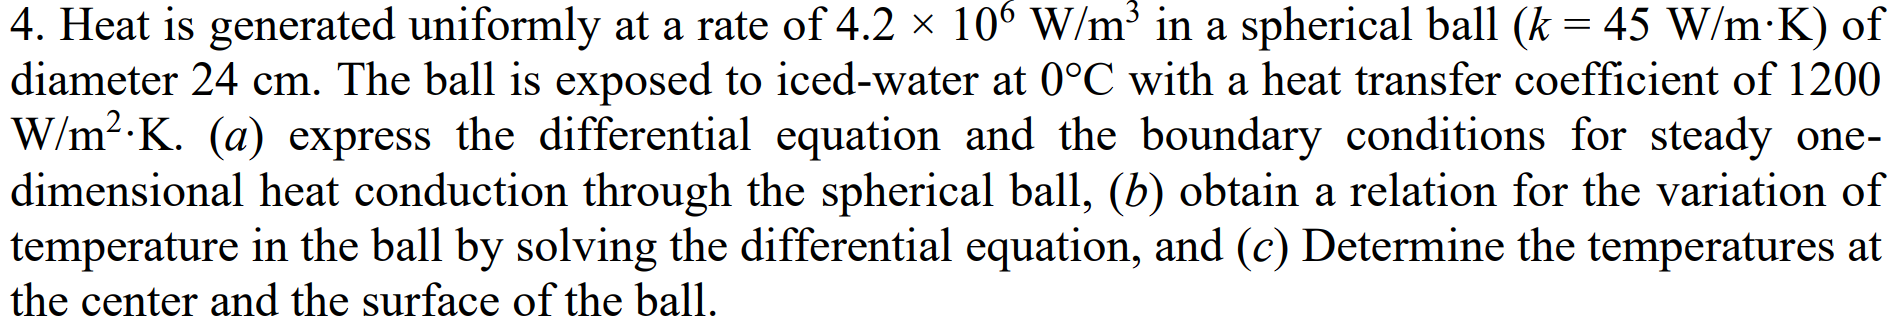
\includegraphics[width=1\textwidth]{problems/p4.png}
    \label{fig:p4}
\end{figure}

\end{document}
